\ifmedium
\begin{frame}[fragile]{Execution and Memory spaces}

  {\Huge Execution and Memory Spaces}

  \vspace{20pt}

  \textbf{Learning objectives:}
  \begin{itemize}
    \item{Heterogeneous nodes and the \textbf{space} abstractions.}
    \item{How to control where parallel bodies are run, \textbf{execution space}.}
    \item{How to control where view data resides, \textbf{memory space}.}
    \item{How to avoid illegal memory accesses and manage data movement.}
    \item{The need for \texttt{Kokkos::initialize} and \texttt{finalize}.}
    \item{Where to use Kokkos annotation macros for portability.}
  \end{itemize}

  \vspace{-20pt}

\end{frame}
\fi

%==========================================================================

%\begin{frame}[fragile]{Execution spaces (0)}
%
%  \textbf{Thought experiment}: Consider this code:
%
%  \vspace{5pt}
%
%  \lstset{mathescape, escapeinside={<@}{@>},
%          language=C,
%          keywords={}}
%
%  \begin{lstlisting}[linebackgroundcolor={
%        \btLstHL{1-3}{darkred!20}
%      }
%    ]
%  MPI_Reduce(...);
%  FILE * file = fopen(...);
%  runANormalFunction(...data...);
%  \end{lstlisting}
%
%  \vspace{-11pt}
%
%  \begin{lstlisting}[linebackgroundcolor={
%        \btLstHL{3-4}{bodyColor}
%      }
%    ]
%  Kokkos::parallel_for(numberOfSomethings,
%                       [=] (const int64_t somethingIndex) {
%                         const double y = ...;
%                         // do something interesting
%                       }
%                       );
%  \end{lstlisting}
%
%  \begin{textblock*}{0.5\textwidth}(0.08\textwidth,0.235\textheight)
%    \rotatebox{90}{{\footnotesize {\color{darkred!80} section 1}}}
%  \end{textblock*}
%
%  \begin{textblock*}{0.5\textwidth}(0.08\textwidth,0.40\textheight)
%    \rotatebox{90}{{\footnotesize {\color{blue!80} section 2}}}
%  \end{textblock*}
%
%  \pause
%
%  \begin{itemize}
%    \item{Where will {\color{darkred!80}section 1} be run?  CPU?  GPU?}
%    \item{Where will {\color{blue!80}section 2} be run?  CPU?  GPU?}
%    \item{How do I \textbf{control} where code is executed?}
%  \end{itemize}
%
%  \pause
%  \vspace{5pt}
%
%  \hspace{20pt}{\Large $\Rightarrow$ \textbf{Execution spaces}}
%
%\end{frame}

%==========================================================================

\begin{frame}{Execution spaces (1)}

  \vspace{-15pt}

  \begin{center}
  \textbf{Execution Space} \\
  a homogeneous set of cores and an execution mechanism \\
  (i.e., ``place to run code'')
  \end{center}

  \vspace{-15pt}

  \begin{center}
    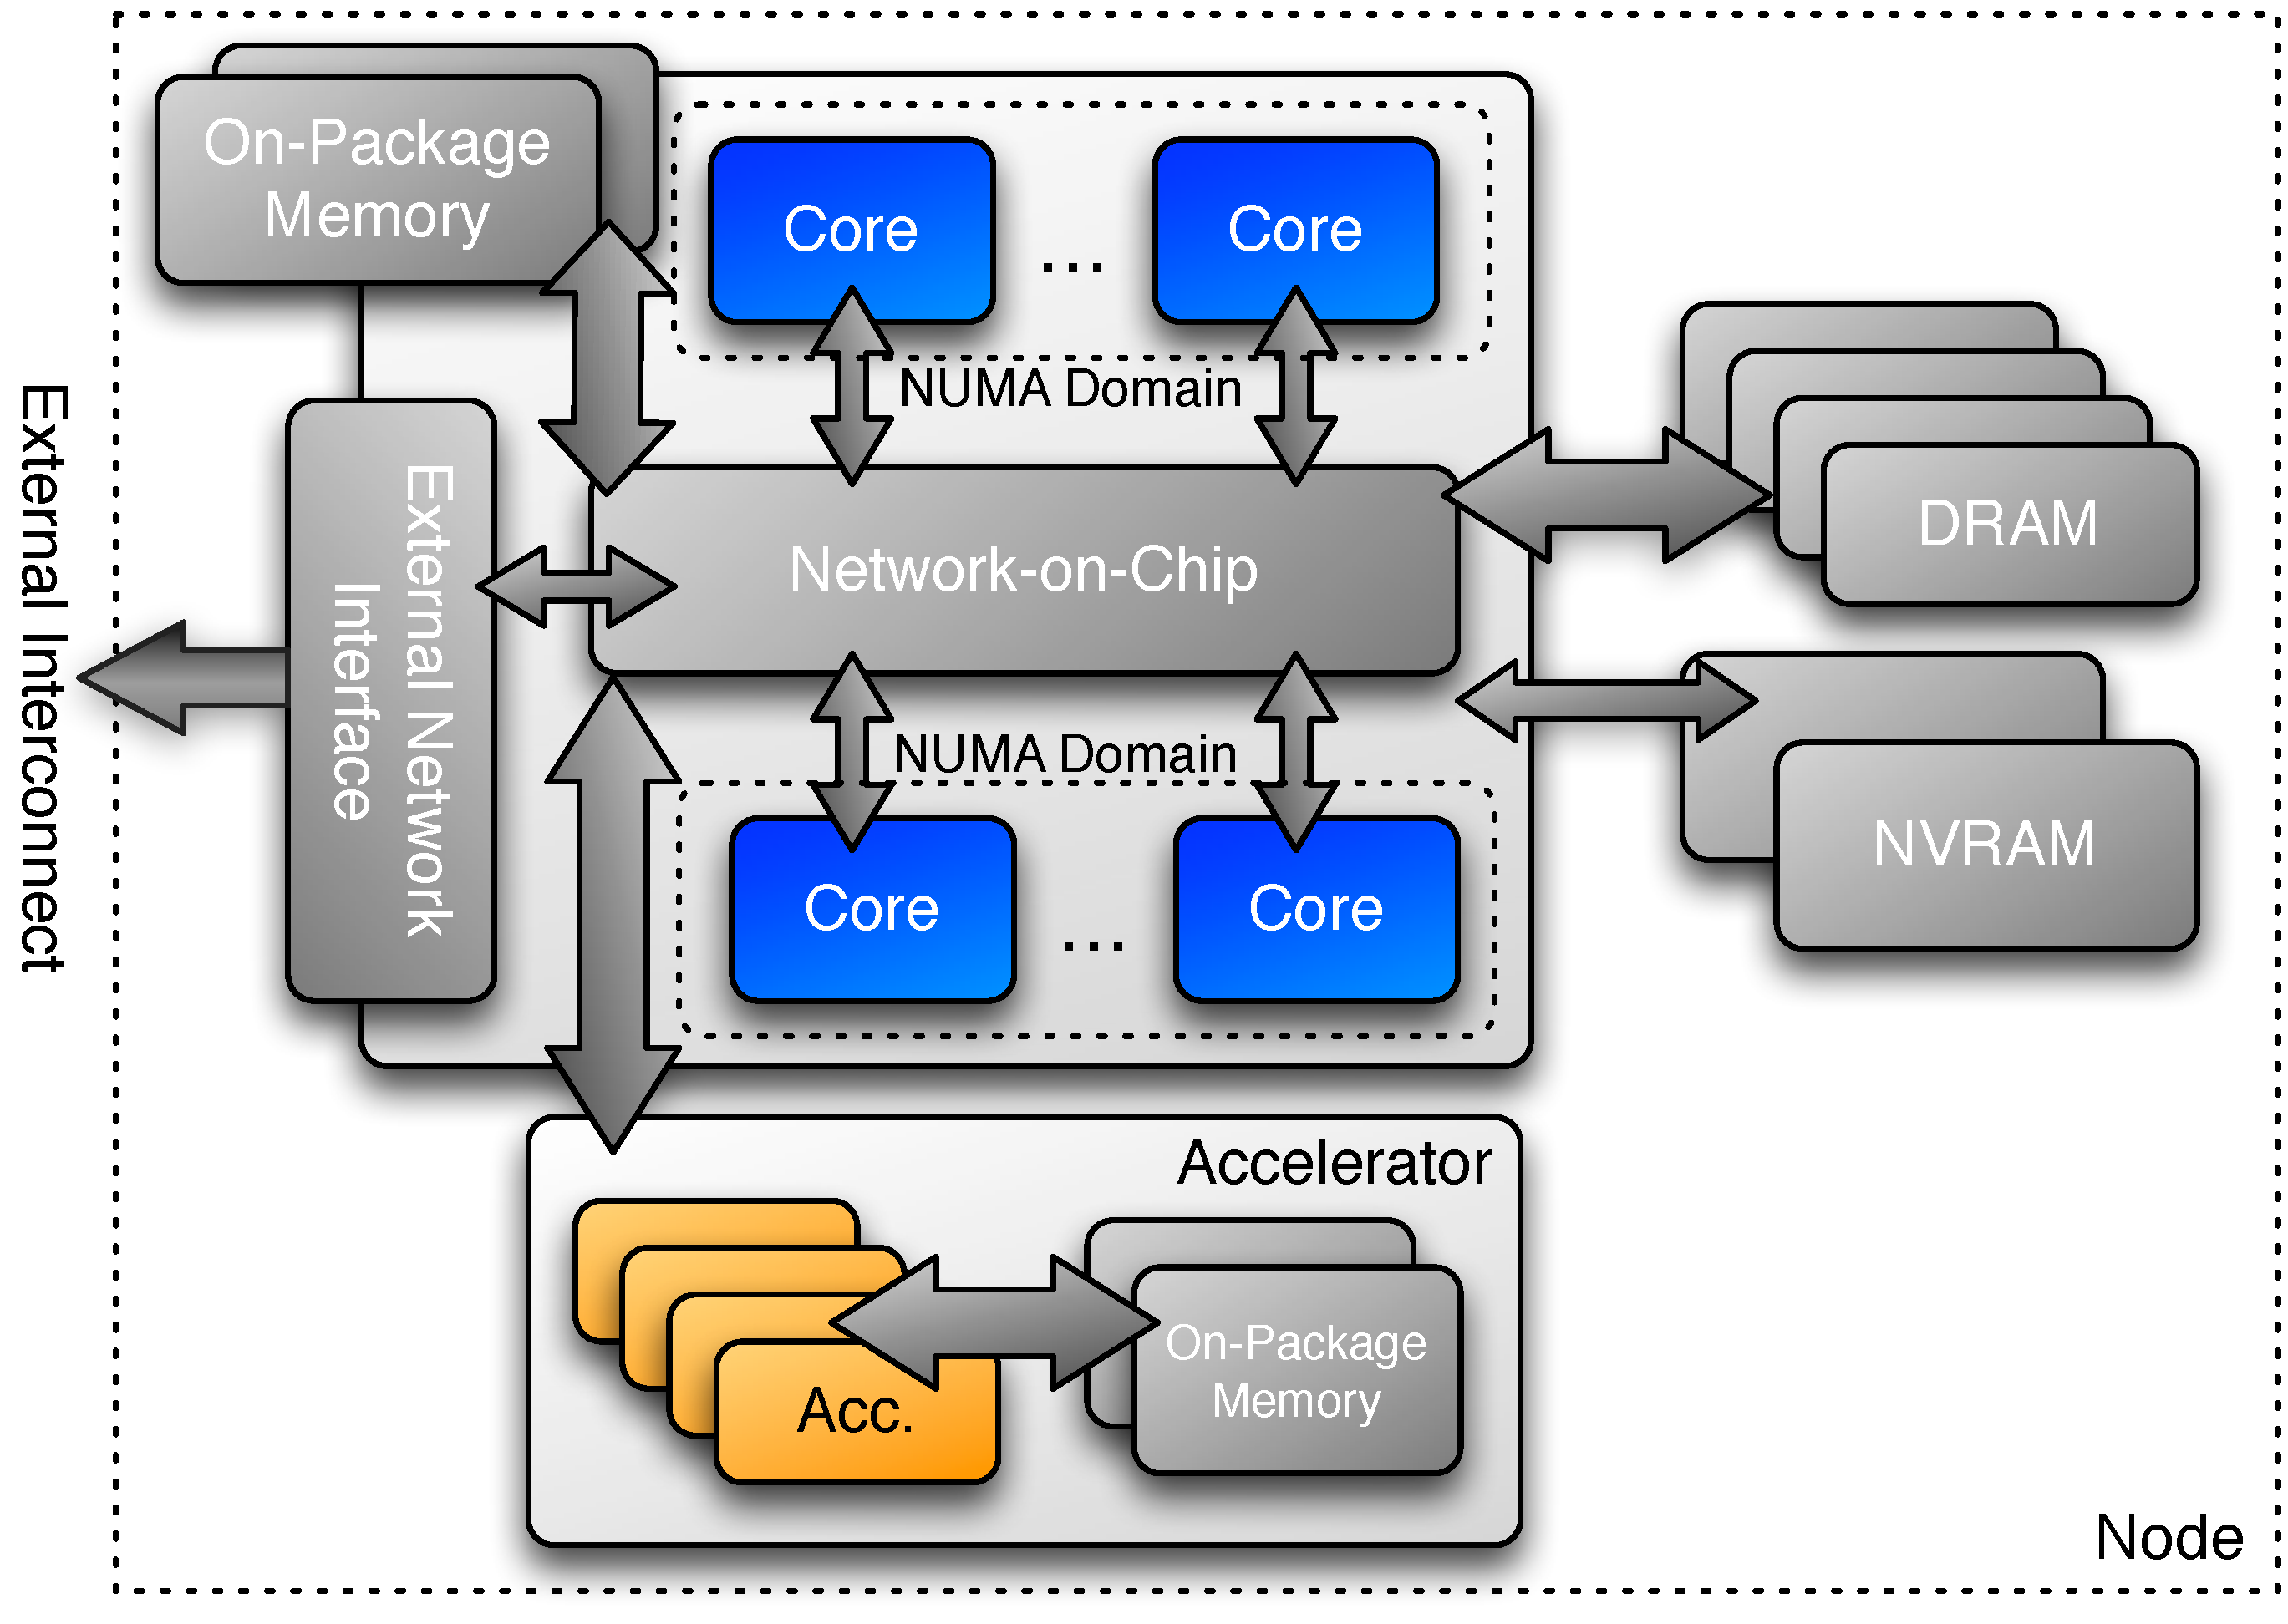
\includegraphics[width=0.70\textwidth]{figures/kokkos-execution-space}
  \end{center}

  \vspace{-12pt}

  {Execution spaces: \texttt{Serial, Threads, OpenMP, Cuda, HIP,} ... }

\end{frame}

%==========================================================================

\ifmedium
\begin{frame}[fragile]{Execution spaces (2)}

  \lstset{mathescape, escapeinside={<@}{@>},
          language=C,
          keywords={}}

  \begin{lstlisting}[linebackgroundcolor={
        \btLstHL{1-3}{darkred!20}
      }
    ]
  MPI_Reduce(...);
  FILE * file = fopen(...);
  runANormalFunction(...data...);
  \end{lstlisting}

  \vspace{-11pt}

  \begin{lstlisting}[linebackgroundcolor={
        \btLstHL{3-4}{bodyColor}
      }
    ]
  Kokkos::parallel_for("MyKernel", numberOfSomethings,
                       [=] (const int64_t somethingIndex) {
                         const double y = ...;
                         // do something interesting
                       }
                       );
  \end{lstlisting}

  \vspace{-5pt}

  \begin{textblock*}{0.5\textwidth}(0.08\textwidth,0.19\textheight)
    \rotatebox{90}{{\footnotesize {\color{darkred!80} Host}}}
  \end{textblock*}

  \begin{textblock*}{0.5\textwidth}(0.08\textwidth,0.315\textheight)
    \rotatebox{90}{{\footnotesize {\color{blue!80} Parallel}}}
  \end{textblock*}

  \pause

  \begin{itemize}
    \item<2->{Where will {\color{darkred!80}Host} code be run?  CPU?  GPU? \\
        \hspace{20pt}{$\Rightarrow$} Always in the \textbf{host process} \\
        \hspace{20pt} also known as \textbf{default host execution space}}
    \item<3->{Where will {\color{blue!80}Parallel} code be run?  CPU?  GPU? \\
      \hspace{20pt}{$\Rightarrow$} The \textbf{default execution space}}
    \item<4->{How do I \textbf{control} where the {\color{blue!80}Parallel} body is executed? \\
      \hspace{20pt}Changing the default execution space (\textit{at compilation}), \\
      \hspace{20pt}or specifying an execution space in the \textbf{policy}.}
  \end{itemize}

\end{frame}
\fi

%==========================================================================

\begin{frame}[fragile]{Execution spaces (3)}

  \textbf{\ul{Changing the parallel execution space:}}

  \vspace{3pt}

  \begin{code}[linebackgroundcolor={
        \btLstHL<1->{4}{bodyColor}
      },
      frame=single
    ]
@patternparallel_for@pattern("Label",
  @policyRangePolicy< @boldExecutionSpace@bold >(0,numberOfIntervals)@policy,
  [=] (const int64_t i) {
    /* ... body ... */
  });
  \end{code}

  \begin{code}[linebackgroundcolor={
        \btLstHL<1->{4}{bodyColor}
      },
      frame=single
    ]
@patternparallel_for@pattern("Label",
  @policynumberOfIntervals@policy, // => RangePolicy<>(0,numberOfIntervals)
  [=] (const int64_t i) {
    /* ... body ... */
  });
  \end{code}

  \begin{textblock*}{0.5\textwidth}(0.05\textwidth,0.465\textheight)
    \rotatebox{90}{\textbf{Default}}
  \end{textblock*}

  \begin{textblock*}{0.5\textwidth}(0.05\textwidth,0.23\textheight)
    \rotatebox{90}{\textbf{Custom}}
  \end{textblock*}

  \pause

  Requirements for enabling execution spaces:
  \vspace{-3pt}
  \begin{itemize}
    \item{Kokkos must be \textbf{compiled} with the execution spaces enabled.}
    \item{Execution spaces must be \textbf{initialized} (and \textbf{finalized}).}
    \item{\textbf{Functions} must be marked with a \textbf{macro} for non-CPU spaces.}
    \item{\textbf{Lambdas} must be marked with a \textbf{macro} for non-CPU spaces.}
  \end{itemize}

\end{frame}

%==========================================================================

\begin{frame}[fragile]{Execution spaces (5)}

  \textbf{\ul{Kokkos function and lambda portability annotation macros:}}

  \vspace{4pt}

  {Function annotation with \texttt{\footnotesize KOKKOS\_INLINE\_FUNCTION} macro}

  \begin{code}[keywords={}, frame=single, basicstyle=\tiny\ttfamily]
@graystruct ParallelFunctor {@gray
  KOKKOS_INLINE_FUNCTION
  @graydouble helperFunction(const int64_t s) const {...}@gray
  KOKKOS_INLINE_FUNCTION
  @grayvoid operator()(const int64_t index) const {
    helperFunction(index);
  }
}@gray
// Where kokkos defines:
#define KOKKOS_INLINE_FUNCTION inline                     // if CPU only
#define KOKKOS_INLINE_FUNCTION inline __device__ __host__ // if CPU + Cuda/HIP
  \end{code}

  \pause

  {Lambda annotation with \texttt{\footnotesize KOKKOS\_LAMBDA} macro}

  \begin{code}[keywords={}, frame=single, basicstyle=\tiny\ttfamily]
@grayKokkos::parallel_for("Label",numberOfIterations, @gray
  KOKKOS_LAMBDA@gray (const int64_t index) {...});@gray

// Where Kokkos defines:
#define KOKKOS_LAMBDA [=]                     // if CPU only
#define KOKKOS_LAMBDA [=] __device__ __host__ // if CPU + Cuda/HIP
  \end{code}

  These macros are \emph{already} defined by Kokkos.

  \vspace{-10pt}

\end{frame}

%==========================================================================

\ifmedium
\begin{frame}[fragile]{Memory Space Motivation}

  \ul{\textbf{Memory space motivating example:} summing an array}

  \begin{code}[linebackgroundcolor={
        \btLstHL<3-4>{3,10}{red!20}
      },
      keywords={}]
View<double*> data("data", size);
for (int64_t i = 0; i < size; ++i) {
  data(i) = ...read from file...
}

double sum = 0;
Kokkos::parallel_reduce("Label",
  RangePolicy<SomeExampleExecutionSpace>(0, size),
  KOKKOS_LAMBDA (const int64_t index, double & valueToUpdate) {
    valueToUpdate += data(index);
  },
  sum);
  \end{code}

  \pause
  \vspace{10pt}

  Question: Where is the data stored? GPU memory?  CPU memory?  Both?

  \pause
  \pause
  \vspace{10pt}

  \hspace{20pt}{\Large $\Rightarrow$ \textbf{Memory Spaces}}

\end{frame}
\fi

%==========================================================================

\begin{frame}[fragile]{Memory spaces (0)}

  \begin{center}
  \textbf{Memory space}: \\
     explicitly-manageable memory resource  \\
     (i.e., ``place to put data'')
  \end{center}

  \vspace{-20pt}

  \begin{center}
    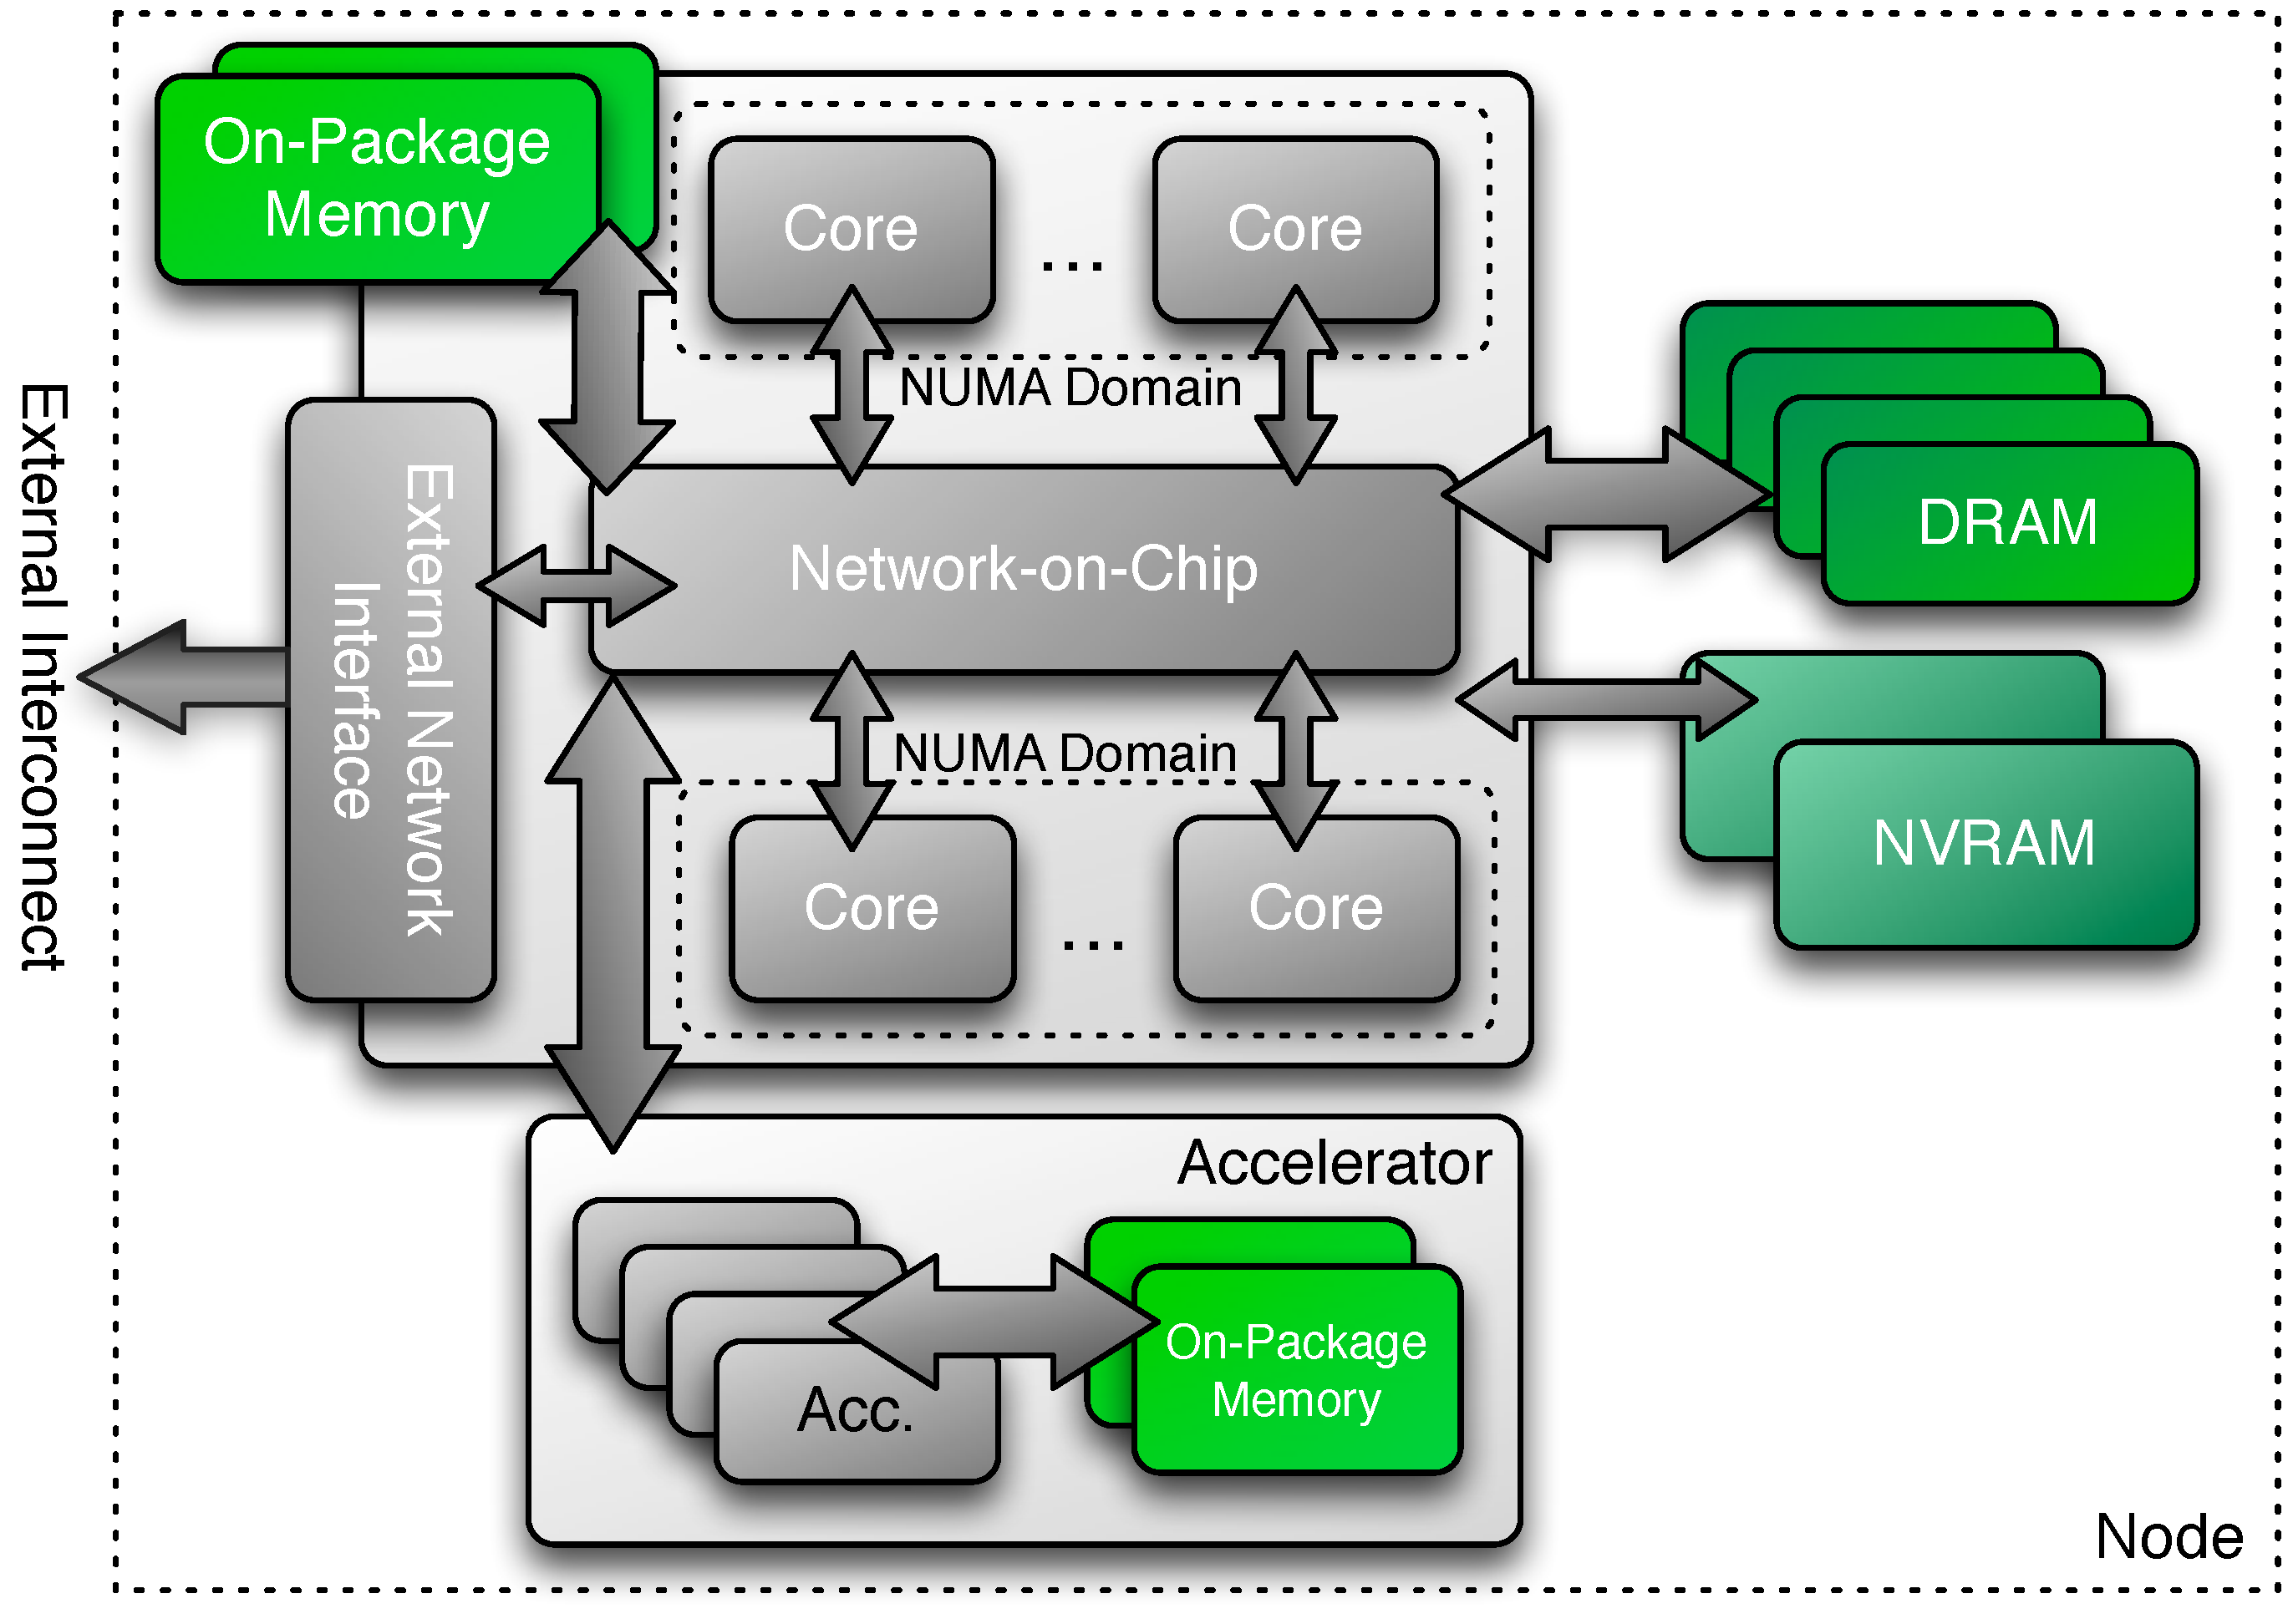
\includegraphics[width=0.75\textwidth]{figures/kokkos-memory-space}
  \end{center}

\end{frame}

%==========================================================================

\begin{frame}[fragile]{Memory spaces (1)}

  \begin{block}{Important concept: Memory spaces}
    Every view stores its data in a \textbf{memory space} set at compile time.
  \end{block}

  \vspace{10pt}

  \begin{itemize}
  \item<2->{\texttt{View<double***,}{\textit{Memory}\textbf{Space}}\texttt{> data(...);}}
  \item<3->{Available \textbf{memory spaces}: \\
            \hspace{20pt}\texttt{HostSpace, CudaSpace, CudaUVMSpace, ...} more} \\
            \hspace{20pt}Portable: \texttt{SharedSpace, SharedHostPinnedSpace}
  \item<4->{Each \textbf{execution space} has a default memory space, which is used if \textbf{Space} provided is actually an execution space}
  \item<5->{If no \texttt{Space} is provided, the view's data resides in the \textbf{default memory space} of the \textbf{default execution space}.}
  \end{itemize}

  \begin{uncoverenv}<6->
  \begin{code}[keywords={View,DefaultExecutionSpace,memory_space}]
  // Equivalent:
  View<double*> a("A",N);
  View<double*,DefaultExecutionSpace::memory_space> b("B",N);
  \end{code}
  \end{uncoverenv}
\end{frame}

%==========================================================================

\begin{frame}[fragile]{Memory spaces (2)}

  \ul{\textbf{Example: HostSpace}}

  \vspace{-3pt}

  \begin{code}[keywords={}]
View<double**, @boldHostSpace@bold> hostView(...constructor arguments...);
  \end{code}

  \vspace{-18pt}

  \begin{center}
    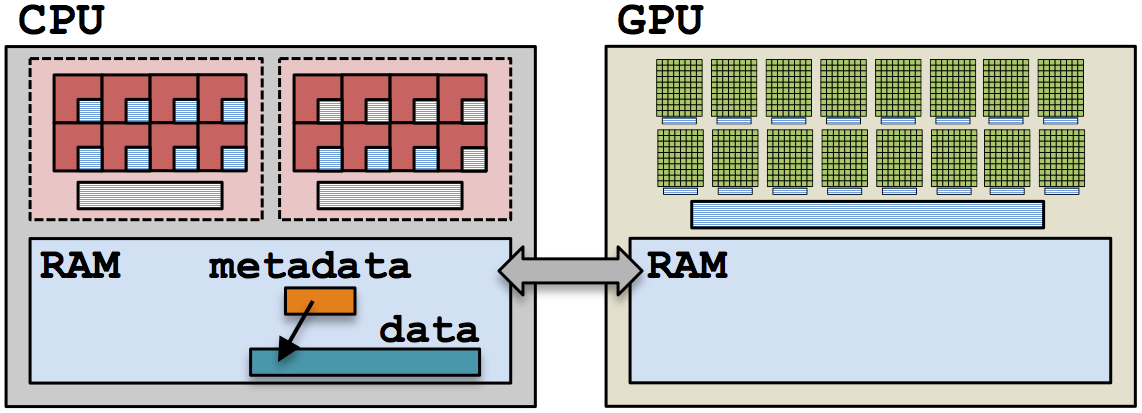
\includegraphics[width=0.70\textwidth]{figures/MemorySpaceExamples_hostSpace}
  \end{center}

  \vspace{-10pt}
  \pause

  \ul{\textbf{Example: CudaSpace}}

  \vspace{-3pt}

  \begin{code}[keywords={}]
View<double**, @boldCudaSpace@bold> view(...constructor arguments...);
  \end{code}

  \vspace{-18pt}

  \begin{center}
    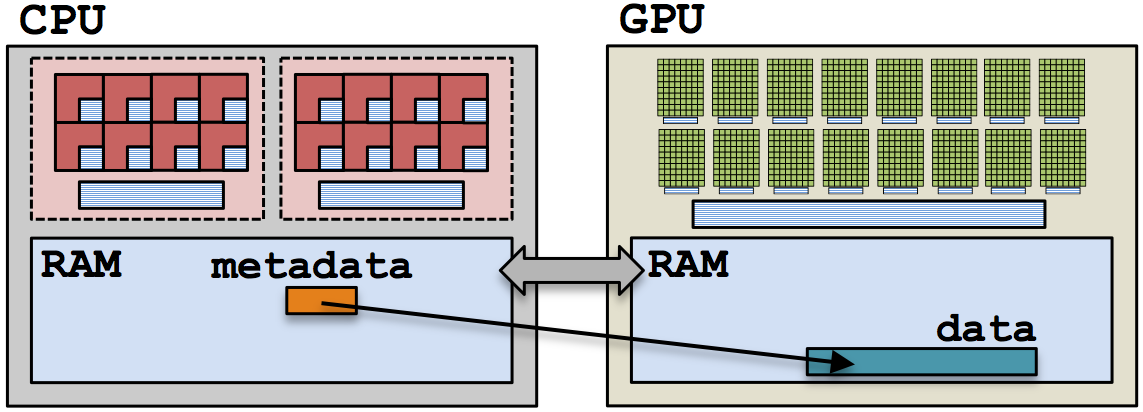
\includegraphics[width=0.70\textwidth]{figures/MemorySpaceExamples_cudaSpace}
  \end{center}

  \vspace{-10pt}

\end{frame}

%==========================================================================

\ifmedium
\begin{frame}[fragile]{Execution and Memory spaces (0)}

  \ul{\textbf{Anatomy of a kernel launch:}}

  \vspace{-10pt}

  \begin{columns}[t,onlytextwidth]

    \column{.6\textwidth}

      \begin{enumerate}
        \item{User declares views, allocating.}
        \item{User instantiates a functor with views.}
        \item{User launches \texttt{parallel\_something}:}
        \begin{itemize}
          \item{Functor is copied to the device.}
          \item{Kernel is run.}
          \item{Copy of functor on the device is released.}
        \end{itemize}
      \end{enumerate}

    \column{.40\textwidth}

      \vspace{10pt}

      \begin{code}[keywords={}]
#define KL KOKKOS_LAMBDA
View<int*, Cuda> @darkgreendev@darkgreen(...);
parallel_for("Label",N,
  KL (int i) {
    @darkgreendev@darkgreen(i) = ...;
  });
      \end{code}

      \vspace{20pt}

  \end{columns}

  \vspace{20pt}

  Note: \textbf{no deep copies} of array data are performed; \\
    \hspace{30pt}\emph{views are like pointers}.

\end{frame}
\fi

%==========================================================================

\ifmedium
\begin{frame}[fragile]{Execution and Memory spaces (1)}

  \begin{columns}[t,onlytextwidth]
    \column{.40\textwidth}

    \vspace{15pt}

    \ul{\textbf{Example: one view}}

    \vspace{5pt}

    \begin{code}[keywords={}]
#define KL KOKKOS_LAMBDA
View<int*, Cuda> @darkgreendev@darkgreen;
parallel_for("Label",N,
  KL (int i) {
    @darkgreendev@darkgreen(i) = ...;
  });
    \end{code}

    \column{.60\textwidth}

      \begin{center}
        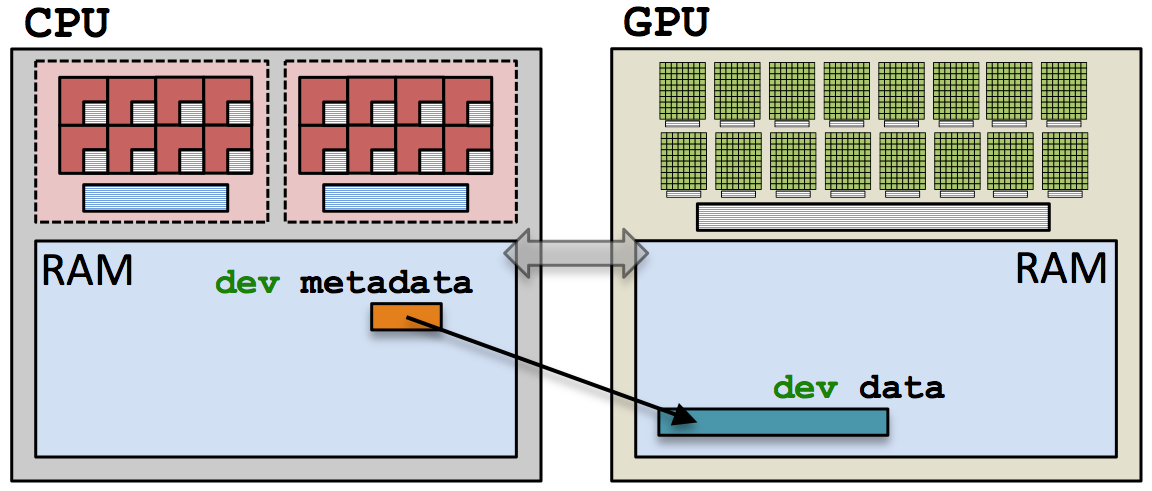
\includegraphics[width=1.00\textwidth]{figures/MemorySpaceExamples_cuda_0}
      \end{center}
      \begin{center}
        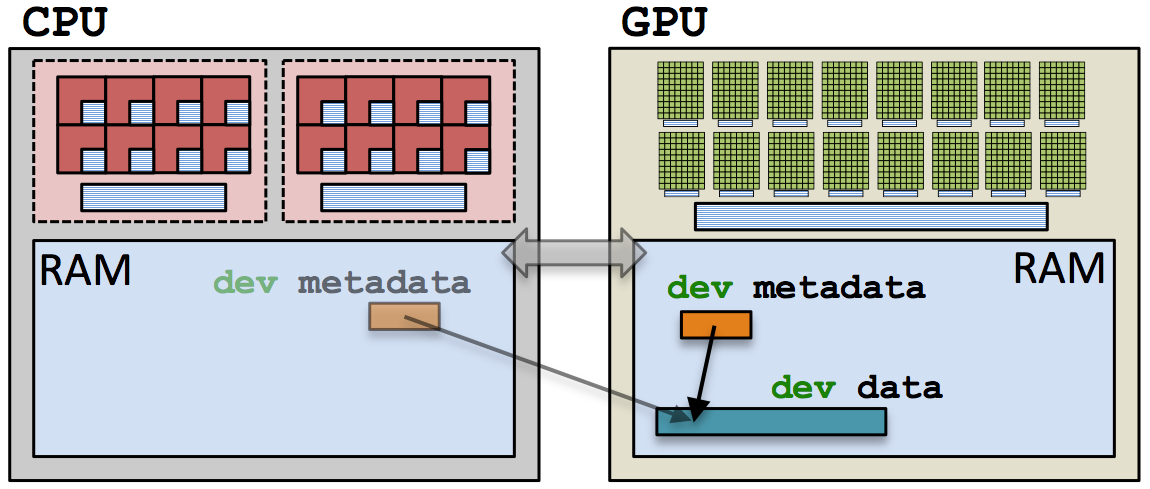
\includegraphics[width=1.00\textwidth]{figures/MemorySpaceExamples_cuda_1}
      \end{center}

  \end{columns}

\end{frame}
\fi

%==========================================================================

\ifmedium
\begin{frame}[fragile]{Execution and Memory spaces (2)}

  \begin{columns}[t,onlytextwidth]
    \column{.40\textwidth}

    \vspace{15pt}

    \ul{\textbf{Example: two views}}

    \vspace{5pt}

    \begin{code}[linebackgroundcolor={
          \btLstHL<2>{7}{red!20}
        },
        keywords={}]
#define KL KOKKOS_LAMBDA
View<int*, Cuda> @darkgreendev@darkgreen;
View<int*, Host> @bluehost@blue;
parallel_for("Label",N,
  KL (int i) {
    @darkgreendev@darkgreen(i)  = ...;
    @bluehost@blue(i) = ...;
  });
    \end{code}

    \column{.60\textwidth}

      \begin{center}
        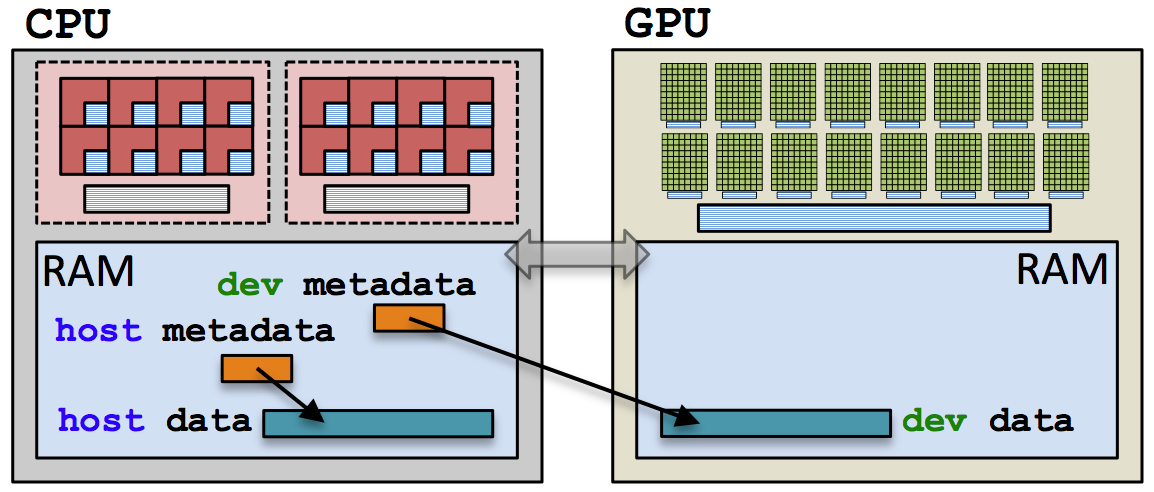
\includegraphics[width=1.00\textwidth]{figures/MemorySpaceExamples_hostCuda_0}
      \end{center}
      \begin{center}
        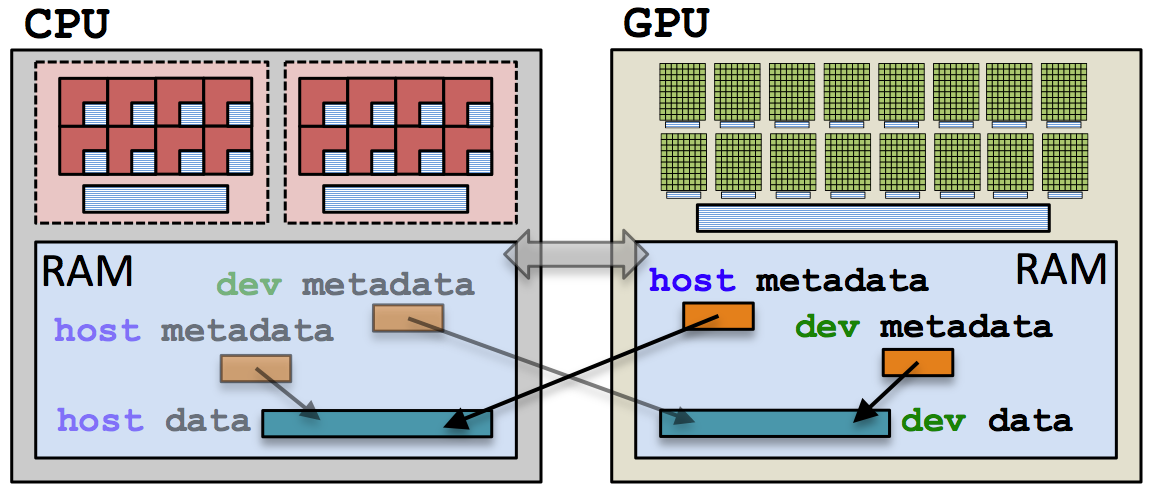
\includegraphics[width=1.00\textwidth]{figures/MemorySpaceExamples_hostCuda_1}
      \end{center}

  \end{columns}

\end{frame}
\fi

%==========================================================================

\begin{frame}[fragile]{Execution and Memory spaces (3)}

  \ul{\textbf{Example (redux): summing an array with the GPU}}

  \vspace{7pt}

  \hspace{10pt}(failed) Attempt 1: \texttt{View} lives in \texttt{CudaSpace}

  \vspace{3pt}

  \begin{code}[linebackgroundcolor={
        \btLstHL<2->{3}{red!20}
      },
      keywords={}]
View<double*, @boldCudaSpace@bold> array("array", size);
@grayfor (int64_t i = 0; i < size; ++i) {@gray
  array(i) = ...read from file...
@gray}@gray

@graydouble sum = 0;@gray
@grayKokkos::parallel_reduce("Label",@gray
  RangePolicy< @boldCuda@bold>(0, size),
  @grayKOKKOS_LAMBDA (const int64_t index, double & valueToUpdate) {@gray
    valueToUpdate += array(index);
  @gray},@gray
  @graysum);@gray
  \end{code}

  \vspace{11pt}

  \begin{textblock*}{0.5\textwidth}(0.94\textwidth,0.382\textheight)
    \only<2->{\texttt{fault}}
  \end{textblock*}

  \vspace{26pt}

\end{frame}

%==========================================================================

\begin{frame}[fragile]{Execution and Memory spaces (4)}

  \ul{\textbf{Example (redux): summing an array with the GPU}}

  \vspace{7pt}

  \hspace{10pt}(failed) Attempt 2: \texttt{View} lives in \texttt{HostSpace}

  \vspace{3pt}

  \begin{code}[linebackgroundcolor={
        \btLstHL<2-3>{10}{red!20}
      },
      keywords={}]
View<double*, @boldHostSpace@bold> array("array", size);
@grayfor (int64_t i = 0; i < size; ++i) {@gray
  array(i) = ...read from file...
@gray}@gray

@graydouble sum = 0;@gray
@grayKokkos::parallel_reduce("Label",@gray
  RangePolicy< @boldCuda@bold>(0, size),
  @grayKOKKOS_LAMBDA (const int64_t index, double & valueToUpdate) {@gray
    valueToUpdate += array(index);
  @gray},@gray
  @graysum);@gray
  \end{code}

  \vspace{3pt}

  \begin{textblock*}{0.5\textwidth}(0.82\textwidth,0.630\textheight)
    \only<2->{\texttt{illegal access}}
  \end{textblock*}

  \pause
  \pause
  \begin{columns}[t,onlytextwidth]
    \column{.35\textwidth}
      What's the solution?
    \column{.65\textwidth}
      \vspace{-25pt}
      \begin{itemize}
        \item{\texttt{SharedSpace}}
        \item{\texttt{SharedHostPinnedSpace} (skipping)}
        \item{Mirroring}
      \end{itemize}
  \end{columns}

\end{frame}

%==========================================================================

\ifmedium
\begin{frame}[fragile]{Execution and Memory spaces (5)}

  \vspace{-30pt}

  \begin{columns}[t,onlytextwidth]
    \column{.40\textwidth}

    \vspace{15pt}

    \ul{\texttt{SharedSpace}}

    \vspace{5pt}

    \begin{code}[keywords={}]
#define KL KOKKOS_LAMBDA
View<double*,
     @boldSharedSpace@bold> @darkgreenarray@darkgreen;
@darkgreenarray@darkgreen = ...from file...
double sum = 0;
parallel_reduce("Label", N,
  KL (int i, double & d) {
    d += @darkgreenarray@darkgreen(i);
  },
  sum);
    \end{code}

    \vspace{5pt}

    %{\color{red}Warning:} \\ \hspace{10pt}Performance penalty

    \column{.55\textwidth}

      \begin{center}
        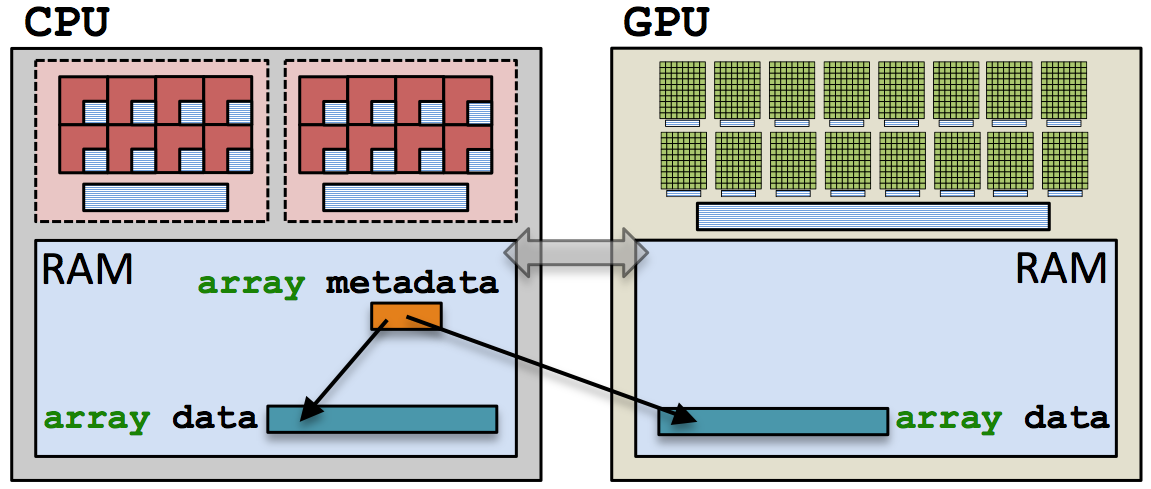
\includegraphics[width=0.95\textwidth]{figures/MemorySpaceExamples_uvm_0}
      \end{center}
      \begin{center}
        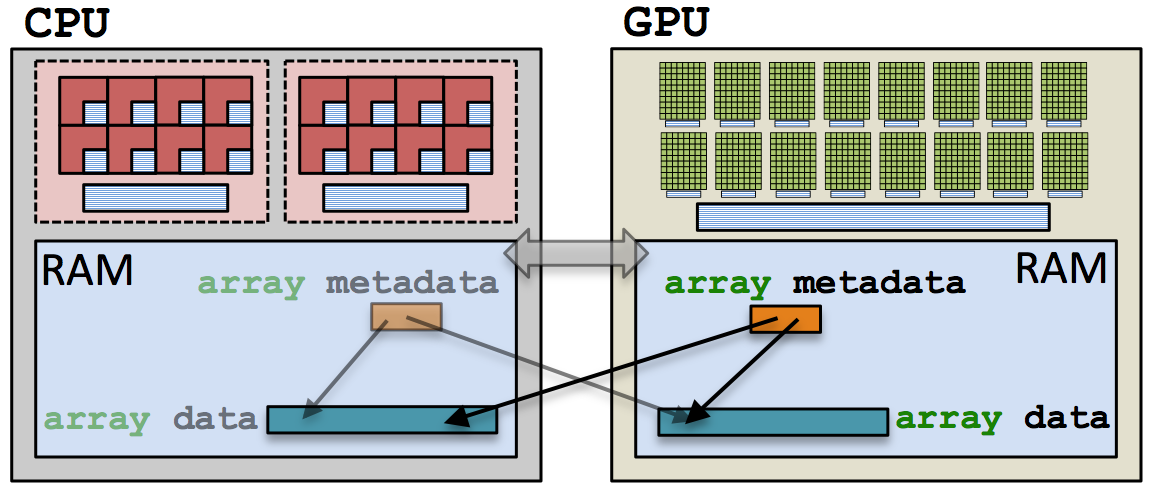
\includegraphics[width=0.95\textwidth]{figures/MemorySpaceExamples_uvm_1}
      \end{center}

  \end{columns}

  \vspace{10pt}

  Cuda runtime automatically handles data movement,
  \\ at a \textbf{performance hit}.

\end{frame}
\fi

\begin{comment}
\begin{frame}[fragile]{Exercise: CG-Solve}

  \textbf{Exercise}: Find $x$ in $b = A * x$

  Getting set up in your home directory:
  \begin{code}
    mkdir Kokkos
    cd Kokkos
    git clone https://github.com/kokkos/kokkos
    git clone https://github.com/kokkos/kokkos-tutorials
  \end{code}

  \vspace{5pt}
  Find the exercise in the kokkos-turoials/Exercises/cg-solve folder.


  \vspace{5pt}
  The Begin subdirectory contains the code. Only cg\_solve.cpp needs modifications.

  \vspace{5pt}
  Look for EXERCISE comments to find places to modify.

\end{frame}

%==========================================================================

\begin{frame}[fragile]{Exercise \#1: include, initialize, finalize Kokkos}

  The \textbf{first step} in using Kokkos is to include, initialize, and finalize:

  \begin{code}
#include <Kokkos_Core.hpp>
int main(int argc, char* argv[]) {
  /* ... do any necessary setup (e.g., initialize MPI) ... */
  Kokkos::initialize(argc, argv);
  {
  /* ... do computations ... */
  }
  Kokkos::finalize();
  return 0;
}
  \end{code}

  \vspace{7pt}

  (Optional) Command-line arguments or environment variables:

  \vspace{3pt}

	\begin{tabular}{| p{0.5\textwidth} | p{0.5\textwidth} |}
    \hline
	  \texttt{--kokkos-threads=INT} or \texttt{KOKKOS\_NUM\_THREADS} & total number of threads \\
    \hline
	  \texttt{--kokkos-device-id=INT} or \texttt{KOKKOS\_DEVICE\_ID} & device (GPU) ID to use \\
    \hline
  \end{tabular}

\end{frame}

%==========================================================================



\begin{frame}[fragile]{Exercise: Compiling}

\ul{\textbf{Compiling for CPU}}

\vspace{-3pt}
  \begin{small}
  \begin{code}
    cmake -B build_openmp -D Kokkos_ENABLE_OPENMP=ON
    cmake --build build_openmp -j
  \end{code}
  Optional: configure with \texttt{Kokkos\_ARCH\_NATIVE=ON} or specify explicitly the target architecture
  \end{small}

%  \hspace{10pt} {\tiny \url{https://github.com/kokkos/kokkos/wiki/Compiling#table-43-architecture-variables}}

\ul{\textbf{Running on CPU} with OpenMP back-end}

\vspace{-3pt}
  \begin{small}
  \begin{code}
  # Set OpenMP affinity
  export OMP_NUM_THREADS=8
  export OMP_PROC_BIND=spread OMP_PLACES=threads
  # Print example command line options:
  ./cg\_solve.exe -h
  # Run with defaults on CPU
  ./cg\_solve.exe
  # Run larger problem
  ./cg\_solve.exe 200 200
  \end{code}
  \end{small}

\ul{\textbf{Things to try:}}
  \begin{small}
  \begin{itemize}
  \itemsep0em
  \item Vary number of threads
  \item Vary problem size
  \item Compare Serial backend performance to unmodified code
  \end{itemize}
  \end{small}
\end{frame}

\begin{frame}[fragile]{Exercise: Compiling}

\ul{\textbf{Compiling for GPU}}

\vspace{-3pt}
  \begin{small}
  \begin{code}
    cmake -B build_openmp -D Kokkos_ENABLE_OPENMP=ON
    cmake --build build_openmp -j
  \end{code}
  Optional: configure with \texttt{Kokkos\_ARCH\_NATIVE=ON} or specify explicitly the target architecture
  \end{small}

%  \hspace{10pt} {\tiny \url{https://github.com/kokkos/kokkos/wiki/Compiling#table-43-architecture-variables}}

\ul{\textbf{Things to try:}}
  \begin{small}
  \begin{itemize}
  \itemsep0em
  \item Vary number of iterations
  \item Vary problem size
  \item Compare performance to CPU runs? What is the ratio compared to expected bandwidth ratio?
  \end{itemize}
  \end{small}
\end{frame}
\end{comment}

%==========================================================================
%==========================================================================

\begin{frame}[fragile]{Views, Spaces, and Mirrors}

  \begin{block}{Important concept: Mirrors}
    Mirrors are views of equivalent arrays residing in possibly different memory spaces.
  \end{block}

  \vspace{3pt}
  \pause

  \ul{\textbf{Mirroring schematic}}

  \vspace{-3pt}

  \begin{code}[keywords={view_type}]
Kokkos::View<double**, @boldSpace@bold> @darkgreenview@darkgreen(...);
auto @darkredhostView@darkred = @boldKokkos::create_mirror_view@bold(@darkgreenview@darkgreen);
  \end{code}

  \vspace{-8pt}

  \begin{center}
    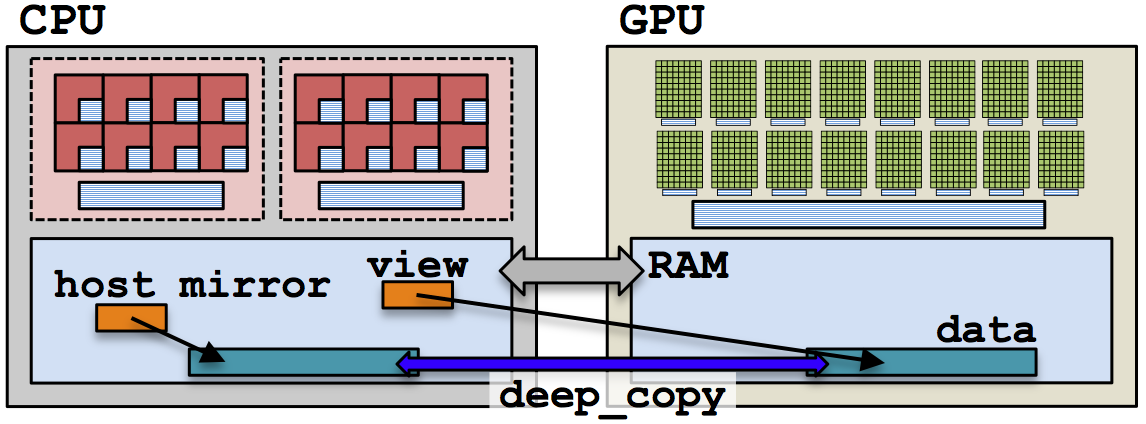
\includegraphics[width=0.70\textwidth]{figures/MemorySpaceExamples_mirrors}
  \end{center}

  \vspace{-10pt}

\end{frame}

%==========================================================================

\begin{frame}[fragile]{Mirroring pattern}

  \begin{enumerate}
    \item<+->{\textbf{Create} a {\color{darkgreen}\texttt{view}}'s array in some memory space. \\

      \vspace{-5pt}
      \begin{code}[keywords={view_type}]
  Kokkos::View<double*, @boldSpace@bold> @darkgreenview@darkgreen(...);
      \end{code}
      \vspace{-4pt}

  }
    \item<+->{\textbf{Create} {\color{darkred}\texttt{hostView}}, a \textit{mirror} of the {\color{darkgreen}\texttt{view}}'s array residing in the host memory space. \\

      \vspace{-5pt}
      \begin{code}[keywords={view_type}]
  auto @darkredhostView@darkred = @boldKokkos::create_mirror_view@bold(@darkgreenview@darkgreen);
      \end{code}
      \vspace{-4pt}

  }
    \item<+->{\textbf{Populate} {\color{darkred}\texttt{hostView}} on the host (from file, etc.).}
    \item<+->{\textbf{Deep copy} {\color{darkred}\texttt{hostView}}'s array to {\color{darkgreen}\texttt{view}}'s array. \\

      \vspace{-5pt}
      \begin{code}[keywords={}]
  Kokkos::@bolddeep_copy@bold(@darkgreenview@darkgreen, @darkredhostView@darkred);
      \end{code}
      \vspace{-4pt}

  }
    \item<+->{\textbf{Launch} a kernel processing the {\color{darkgreen}\texttt{view}}'s array. \\

      \vspace{-5pt}
      \begin{code}[keywords={}]
  Kokkos::parallel_for("Label",
    RangePolicy< @boldSpace@bold>(0, size),
    KOKKOS_LAMBDA (...) { use and change @darkgreenview@darkgreen });
      \end{code}
      \vspace{-4pt}

  }
    \item<+->{If needed, \textbf{deep copy} the {\color{darkgreen}\texttt{view}}'s updated array back to the {\color{darkred}\texttt{hostView}}'s array to write file, etc. \\

      \vspace{-5pt}
      \begin{code}[keywords={}]
  Kokkos::@bolddeep_copy@bold(@darkredhostView@darkred, @darkgreenview@darkgreen);
      \end{code}
      \vspace{-4pt}

  }
  \end{enumerate}

\end{frame}

%==========================================================================

\begin{frame}[fragile]{Mirrors of \texttt{View}s in \texttt{HostSpace}}

  What if the \texttt{View} is in \texttt{HostSpace} too?  Does it make a copy?

  \begin{code}[keywords={}]
Kokkos::View<double*, @boldSpace@bold> @darkgreenview@darkgreen("test", 10);
auto @darkredhostView@darkred = @boldKokkos::create_mirror_view@bold(@darkgreenview@darkgreen);
  \end{code}

  \begin{itemize}
    \item{\texttt{create\_mirror\_view} allocates data only if the host process cannot access {\color{darkgreen}view}'s data, otherwise {\color{darkred}hostView} references the same data.}
    \item{\texttt{create\_mirror} \textbf{always} allocates data.}
    \item{\texttt{create\_mirror\_view\_and\_copy} allocates data if necessary and also \textbf{copies} data.}
  \end{itemize}

  Reminder: Kokkos \emph{never} performs a \textbf{hidden deep copy}.

  \vspace{-5pt}

\end{frame}

%==========================================================================

\begin{frame}[fragile]{Exercise \#3: Flat Parallelism on the GPU, Views and Host Mirrors}

  \textbf{Details}:
  \begin{scriptsize}
  \begin{itemize}
\item Location: \ExerciseDirectory{03/Begin}
\item Add HostMirror Views and deep copy
\item Make sure you use the correct view in initialization and Kernel
\end{itemize}
  \end{scriptsize}

\begin{code}
  # Compile for CPU
  cmake -B build_openmp -DKokkos_ENABLE_OPENMP=ON
  cmake --build build_openmp
  # Run on CPU
  ./build_openmp/03_Exercise -S 26
  # Note the warnings, set appropriate environment variables
  # Compile for GPU
  cmake -B build_cuda -DKokkos_ENABLE_CUDA=ON
  cmake --build build_cuda
  # Run on GPU
  ./build_cuda/03_Exercise -S 26
\end{code}

  \ul{\textbf{Things to try:}}
  \begin{scriptsize}
  \begin{itemize}
  \item Vary problem size and number of rows (-S ...; -N ...)
  \item Change number of repeats (-nrepeat ...)
  \item Compare behavior of CPU vs GPU
  \end{itemize}
  \end{scriptsize}



\end{frame}

%==========================================================================

\begin{frame}[fragile]{View and Spaces Section Summary}

  \begin{itemize}
    \item{Data is stored in \texttt{Views} that are ``pointers'' to \textbf{multi-dimensional arrays} residing in \textbf{memory spaces}.}
    \item{\texttt{Views} \textbf{abstract away} platform-dependent allocation, (automatic) deallocation, and access.}
    \item{\textbf{Heterogeneous nodes} have one or more memory spaces.}
    \item{\textbf{Mirroring} is used for performant access to views in host and device memory.}
    \item{Heterogeneous nodes have one or more \textbf{execution spaces}.}
    \item{You \textbf{control where} parallel code is run by a template parameter on the execution policy, or by compile-time selection of the default execution space.}
  \end{itemize}

\end{frame}
